%!TEX root = ../main.tex
\section{New Protocol}

\input{Sections/additionalDetails}

%TODO: here we should describe the protocols implemented
%should be rewritten

%TOOO: put after background
\section{Preliminaries}
We begin by defining some basic notations that we will use throughout this work. We use uppercase letters (e.g.,
A, B) to denote matrices and bold letters to denote vectors \textbf{a} . As was specified in the Boneh et al work \cite{darkmatter}, the input variables to the PRF functions are the key ${K}$ which is of size $m \times n$ and each input vector $\textbf{i}$ of size $n$. 
To save on bandwidth in the distributed implementation, the key was implemented as a Toeplitz matrix, requiring $m + n - 1$ bits.
At the end of the algorithm, a randomization matrix $R$ is used which is of size $t \times m = 81 \times 256$, resulting in entropy of 128 bits (as $81 = 128 \times \log_2 3$).


\section{Implementation}
\label{sec:technical_overview}

The pre-shared randomness was generated centrally (as if its generated by a third trusted party). Only the online part was implemented in a distributed manner. 

%%%%%%%%%%%%%%%%%%%%%%%%%%%%%%%%%%%%%%%%%%%%%%%%%


\subsection{representing $Z_2$ vector}

The dark matter function manipulates elements of $Z_2$ and $Z_3$. However, machine words can hold up to 64 bits and we use this to represent many elements in just a few machine words, using bit slicing. Namely, we used each machine word as a vector of 64 bits and applied operations to this bit-vector in a SIMD manner.
Since in our implementation each key $\textbf{K}$  is of size $m \times n = 256 \times 256$ and each input is a vector of size $n = 256$, this results in packing each key o $256 \dfrac 64 = 4$ words and each input vector into 4 words. This may result in time saving of up to $\times 64$ of the run-time.

\subsection{Representing $Z_3$ vector}

The last part of the dark matter function takes an intermediate vector viewed as a vector of $Z_3$ elements, which is then multiplied 
by a matrix $R$ in $Z_3$ to produce the output vector in $Z_3$. We tried different methods for implementing this matrix-vector multiplication over $Z_3$.:	

\subsubsection{Bit slicing} Bit slicing is implemented  by representing a vector over $Z_3$  as two binary vectors - one LSB's and one MSB's. The operations over this $Z_3$ vector - addition, subtraction, multiplication and MUX  - were implemented in a bitwise manner as shown in table \ref{tab:multicol}. We took advantage of the fact that when representing each vector as MSB and LSB, negation (which is the same as multiplying by two) is the same as swapping the most and least significant bits. 


% TODO: replace with a table - COMPLETED



\begin{table}[ht]
\caption{Operations in $Z_3$. input:   ${l_1}, {m_1}$ - LSB and MSB  of first trinary number, 
	${l_2}, {m_2}$ - LSB and MSB  of second trinary number,  ${s}$ - selection bit for MUX}
\begin{center}
\begin{tabular}{|c|l|}
    \hline
    \textbf{Operations} & \textbf{Methods}\\
    \hline
    \multirow{3}{*}{Addition} & ${t} := ({l_1 \wedge m_2}) \oplus ({l_2 \wedge m_1})$\\
    & $m_{\mathrm{out}} := ( l_1 \wedge  l_2 ) \oplus  t $ \\
    & $l_{\mathrm{out}} :=m_1 \wedge m_2 ) \oplus t $ \\
    \hline
    \multirow{3}{*}{Subtraction} & ${t} := ({l_1} \wedge {l_2}) \oplus ({m_2} \wedge {m_1})$;\\
    & $m_{\mathrm{out}} := (l_1 \wedge m_2 ) \oplus t$;\\
    & $l_{\mathrm{out}} := (m_1 \wedge l_2 ) \oplus t$; \\
    \hline
\multirow{3}{*}{Multiplication} & $m_{\mathrm{out}}:= (l_1 \vee m_2) \wedge   (m_1 \vee l_2)$; \\
    & $l_{\mathrm{out}} := (l_1 \vee l_2) \wedge     (m_1 \vee m_2)$;\\
    \hline
\multirow{3}{*}{MUX} & $m_{\mathrm{out}} :=( m_2 \vee s) \wedge (m_1 \vee (\bar{s}) )$; \\
    & $l_{\mathrm{out}}[i] :=( l_2 \vee s) \wedge (l_1 \vee (\bar{s}) )$; \\
    \hline

\end{tabular}
\end{center}
\label{tab:multicol}
\end{table}

\iffalse

\subsubsection{Integer packing  operations} Another method that was explored for optimization was integer packing. 
Since in our case we need to multiply a $Z_3$ vector of dimension $m=256$ by a trinary matrix, then each entry in the result can be as large as $256 \times 4 = 1024$, but not larger.
We therefore allocated 10 bits for each entry (capable of holding numbers between 0 and 1023), so we can pack such numbers into each word. Specifically, the vector $(X_0 ... X_5)$ over $Z_3$ is represented as the integer $y = \sum_{i=0}^6 512^i \times x_i$.

When performing the matrix-vector multiplication, multiple rows the matrix were packed using integer-packing. 
%Specifically, the matrix was divided into two matrices of size $81 \times 128$. 
Specifically, the matrix was divided into packs of 6 items each belonging to the same column and  consecutive rows, i.e.,  $R_{i,j}$ where ${i = (6 \times l) ... (6 \times l + 5)}$ were packed into one word, resulting in two matrices of size $14 x 256$. The matrix was then multipled by the trinary vector. The results was divided into consecutive items of 10 bits each and the value $\mod 3$ was calculated as the result
%TODO: write how the matrix was packed but the vector was not

\fi


%TODO: IS THIS CORRECT? CHECK AND CORRECT

\subsubsection{Matrix multiplication using a lookup table}

Even with bitslicing, implementing the matrix-vector multiplication column by column via the opertions from Table~1 is still rather slow.
To get better performence, we capitalized on the fact that the random matrix $R$ is fixed, and we can therefore set up $R$-dependent tables and use table lookups in the implementation of the multiply-by-$R$ operation.

Specifically, we partition the matrix $R$ (which has $m=256$ columns) into sixteen slices of 16 columns each, denoted $R_1,\ldots,R_{16}$.
For each of these small matrices $R_i$, we then build a table with $2^{16}$ entries, holding the result of multiplying $R_i$ by every vector from $\{0,1\}^{16}$.
Namely, let $R_{i,0},R_{i,1},\ldots,R_{i,15}$ be the sixteen columns of the matrix $R_i$.
The table for $R_i$ is then defined as follows: For each index $0\le j < 2^{16}$, let $\vec{J}=(j_0,j_1,\ldots,j_{15})$ be the 0-1 vector holding the bits in the binary representation of~$j$, then we have
\[
T_i[j] = R_i \times \vec{J} = \sum_{k=0}^{15} R_{i,k} \cdot j_k ~~\bmod 3.
\]
Recalling that $R$ is $Z_3$ matrix of dimension $81\times 256$, every entry in each table~$T_i$ therefore holds an 81-vector over $Z_3$.
Specifically, it holds a packed-$Z_3$ element with four words (two for the MSBs and two for the LSBs of this 81-element vector).

Note, however, that $T_i$ can only be used directly to multiply $R_i$ by \emph{0-1 vectors}.
To use $T_i$ when multiplying $R_i$ by a $\{0,1,2\}$ vector, multiply $R_i$ separately by the MBSs and the LSBs of that vector, and then subtract one from the other using the operations from Table~1.
To multiply a dimension-256 $\{0,1,2\}$ vector by the matrix $R$, we partition it into sixteen vectors of dimension 16, use the approach above to multiply each one of them by the corresponding $R_i$, then use the operations from Table~1 to add them all together.
Hence we have

\begin{tabbing}
	\underline{Multiply-by-$R$(input: $\vec{V}\in\{0,1,2\}^{256}$:}\\
	~~1. $Acc := 0$\\
	~~2. For \=$i=0,\ldots,15$\\
	~~3. \> Let $\vec{M}_i,\vec{L}_i\in\{0,1\}^{16}$ be the MSB, LSB vectors (resp.) of $\vec{V}_i=\vec{V}[16i,\ldots,16i+15]$\\
	~~4. \> Set the indexes $m:=\sum_{k=0}^{15}2^i\cdot\vec{M}[i]$
	and $\ell:=\sum_{k=0}^{15}2^i\cdot\vec{L}[i]$\\
	~~5. \> $Acc := Acc + T_i[\ell] - T_i[\ell] \bmod 3$\\
	~~6. Output $Acc$
\end{tabbing}

We note that a sligtly faster implementation could be obtained by braking the matrix into (say) 26 slices of upto 10 columns each, and directly identify each 10-vector over $\{0,1,2\}$ with an index $i<3^{10}=59049$.
This implementation would have only 26 lookup operations instead of 32 in the implementation above, so we expect it to be about 20\% faster. On the other hand it would have almost twice the table size of the implementation from above.

\section{Analysis}

Table \ref{CommunicationCosts} includes the computation and communication results for the different protocol.

% Table: Communication Cost
\begin{table}[htbp]
	\label{CommunicationCosts}
	%[h]
	\begin{center}
		%\begin{minipage}{10cm}
		\begin{tabular}{|c|c|c|c|c|}
			\hline
			 \multicolumn{1}{|p{5cm}|}{\centering Protocol}
			& \multicolumn{1}{|p{2cm}|}{\centering Round  \\Complexity}
			& \multicolumn{1}{|p{3cm}|}{\centering Online \\ Communication}
			& \multicolumn{1}{|p{3cm}|}{\centering Preprocessing \\ Size}
			& \multicolumn{1}{|p{3cm}|}{\centering Computation \\ Operation}\\
			\hline
			\hline

			\textbf{Centralized WPRF} & - & - & - & 9K\\
			\hline
			\textbf{Distributed WPRF \cite{darkmatter} } & 4 & 5 & 2K &  45K\\
			\hline

			\textbf{Our WPRF  } & 3 & 5 & 1M &  13K\\
			\hline

			\textbf{Our OPRF } & 3 & 5 & 1M & 11K\\

			\hline
			
		\end{tabular}
		
		\vspace{-1mm}
		\caption{Communication Analysis of different protocols. The protocols were optimized using both the bit packing and the lookup table}
		%\end{minipage}
	\end{center}
	\vspace{-5mm}
\end{table}


\section{Benchmarking}

We compare our run-time to discrete-log based PRFs. To this end, we use the lib sodium library \cite{LibSodium}. The library uses elliptic curve 252 bits, and includes a function that performs scalar multiplication ('crypto\_scalarmult\_ed25519').


\section{Experimental Results}

The system was tested using Ubuntu Server 18.04 on a t2.medium AWS environment. To record the timings, the code was run in a loop 1000 times. Below are run-time results for running a single instance of PRF in microsecond. The results include both centralized and distributed versions of the PRF. In order to increase efficiency, packing and lookup tables were used. The packing indicates both the $Z_2$ and $Z_3$ packing.

%add table
\begin{table}[htbp]
	%[h]
	\begin{center}
		%\begin{minipage}{10cm}
		\begin{tabular}{|c|c|c|c|c|c|}
			\hline
			\textbf{Protocol} & \textbf{Packed }  &  \textbf{lookup} & \textbf{Runs/sec} & \textbf{Runtime($\mu$ sec)}\\
			\hline
			\hline
			\textbf{Centralized wPRF}  & N  & N  &  50K&20.2 \\
			\hline
			\textbf{Centralized wPRF} & Y  &  N & 65.4K &18.5  \\
			\hline
			\textbf{Centralized wPRF(int pack)} & Y  &  N & 84K &11.85 \\
			\hline
			\textbf{Centralized wPRF} & Y  &  Y & 165K &6.08 \\
			\hline
			
		\end{tabular}
		
		\vspace{-1mm}
		\caption{Comparison of the run-time and computation of the different Optimized Centralized wPRF.}
		\label{CentralRuntimeTable}
		%\end{minipage}
	\end{center}
	\vspace{-5mm}
\end{table}

\begin{table}[htbp]
	%[h]
	\begin{center}
		%\begin{minipage}{10cm}
		\begin{tabular}{|c|c|c|c|}
			\hline
			\textbf{Protocol} & \textbf{Runs/sec} & \textbf{Runtime($\mu$ sec)} \\
			\hline
			\hline
			\textbf{Fully Distributed WPRF\cite{darkmatter}} & 24K & 40.56  \\
			\hline
			\textbf{Fully Distributed WPRF} &  82K &  12.12\\
			\hline
			\textbf{OPRF with lookup} &  104K &  9.52 \\
			\hline
			\textbf{Discrete log-based PRF } & 12K &\textbf{86.07}\\
			\hline
			
		\end{tabular}
		
		\vspace{-1mm}
		\caption{Optimized protocols runtime. These protocols utilize both the bit-packing and lookup table optimization}
		\label{RuntimeTable}
		%\end{minipage}
	\end{center}
	\vspace{-5mm}
\end{table}

%%%%%%%%%%%%%%%%%%%%%%%%%%%%

\iffalse

In this work we implemented a few distributed protocols of the PRF introduced by Boneh et. Al  \cite{darkmatter}:

$PRF_k(x) = R \times (K \times x \mod 2)  \mod 3 $

where $R$ is a randomization matrix in $Z_3$, $K$ is an $m \times n$ key and $x$ is an $n$-length vector. Specifically, we present a new protocol for implementing this PRF. The protocol uses a shared input and output which provides improved performance over the original protocol described in \cite{darkmatter}. For context, we also implement the original protocol \cite{darkmatter} . We also introduce an improved OPRF (Oblivious PRF) protocol, in which one party has the input and one has the key. Below are  details of the protocols.

\subsection{PRF}


\paragraph{notations:} below are the notations we use to describe the protocols: \\
$K$ is the key, represented by an $m \times n$ matrix \\
$x$ is the input, represented by an $n$ size vector \\
$R_x, r_k$ - pre-shared randomness for key $K$ and input $x$ \\
$r$ - random vector in $Z_3$]
We use capital letters for matrices, and $\vec{x}$ notation for vectors \\

\section{Appendix}

\paragraph{Original - Distributed Input Distributed Output (DIDO) - WPRF Protocol}

The protocol was introduced in \cite{darkmatter}. The main details of the protocols are described below (\ref{2PartyDarkMatter}). In this setting, both the input and the key are secret shared additively between the two parties. Both the protocol presented in this paper and the original protocol are two-party PRFs. For our implementation, randomization was added in phase 3 to provide $Z_3$ output with 128-bit entropy. 
The protocol is described in \figref{algorithm1}.
%add  a description of the protocol

\begin{figure*}[ht]
	\centering
	\includegraphics[width=1.2\textwidth]{images/old_protocol2.pdf}
	\vspace{-2mm}
	\caption{Old wPRF protocol}
	\label{old_protocol.fig}
	\vspace{-5mm}
\end{figure*}


\begin{algorithm}
	\caption{2-Party dark matter WPRF}
	\label{2PartyDarkMatter}
	
	
	Input: ${K_{m\times n} }(i)$ and $\vec{Inp}(i_n)$ key and user input of each user,\\
	$(i = 1...2, n,m = 256)$\\ 
	Output: user 1: $\vec{K} \times x + \vec{r}$\\
	user2: $-  \vec{r}$\\   %SVec = salt vectorx`
	
	\begin{algorithmic}
		
		\STATE \textbf{Preprocessing}:
		
		Output: 	user 1: $\vec{R_a}, \vec{r_b}$ - pre-shared randomness \\
		user 2: $\vec{r_x} $- pre-share randomness \\
		
		\STATE  \textbf{Stage\ 1}: calculate $a \times b \plus c$
		
		input: user 1: ${\vec{A}, \vec{b}, {\vec R_a}, \vec{r_b} } $ \\
		user 2: ${\vec{x}, \vec{r_x},  \vec{z} }$ \\
		
		\begin{enumerate}
			
			\item user 2 $\vec{m_x} = \vec{x} -\vec{r_x}  \rightarrow  $  user 1
			
			\item user 1  $ \leftarrow   \vec{M_a} =  \vec{A} - \vec{r_A}   $ user 2
			
			\item user 2 $ \vec{m_b} = \vec{R_a} \times \vec{m_x} + \vec{b}  - \vec{r_b}  \rightarrow $ user 1
		\end{enumerate}
		
		Output: $user 1: \vec{- b} $  \\
		$user 2: \vec{M_a} \times \vec{x} + \vec{m_b} + \vec{z} = \vec{A} \vec{x} + \vec{b}$ \\
		
		\STATE  \textbf{Stage\ 2}: Oblivious Transfer
		input: 	 user 1:  $\vec{r_1}, \vec{r_2}, \vec{r_a}, \vec{r_b}$ - vectors in $Z_3$
		user 2:  $\vec{x}, \vec{r_x}$ - vectors in $Z_2$, $\vec{z} $ - vector in $Z_3$
		
		
		\begin{enumerate}
			\item user 1  $ \leftarrow   \vec{m_x} = \vec{x} \oplus \vec{r_x}$   user 2
			
			\item user 1:  $  \vec{m_1} = \vec(- m_x)  \vec{r_a} + \vec{m_x} \vec{r_b} + \vec{r_1}   \rightarrow $   user 2
			
			\item user 1:  $  \vec{m_2} = \vec(m_x)  \vec{r_a} + \vec{- m_x} \vec{r_b} + \vec{r_2}  \rightarrow $   user 2
			
			
		\end{enumerate}
		
		output:  user 2: $\vec{w}:= \vec{x} \times \vec{m_2}+ - \vec{x}  \times \vec{m_1} - \vec{z}$
		
		
		\STATE  \textbf{stage 3}: $Z_3$ randomization  
		
	\end{algorithmic}
	
\end{algorithm}




%add table with parameters, including communication

\paragraph{Our improved (DIDO) wPRF protocol}

\begin{figure*}[ht]
	\centering
	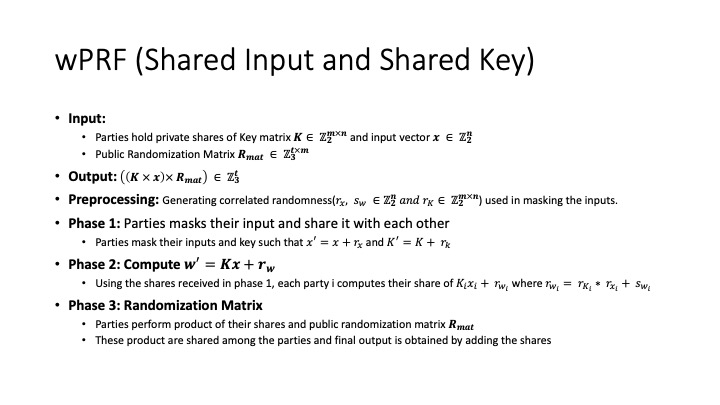
\includegraphics[width=0.8\textwidth]{images/sisk.jpg}
	\vspace{-2mm}
	\caption{Distributed Input Distributed Output wPRF protocol}
	\label{sisk.fig}
	\vspace{-5mm}
\end{figure*}

\begin{algorithm}
	\caption{2-Party Distributed PRF (Shared input and Shared Key)}
	\begin{algorithmic}
		\STATE Input: $x \in \mathbb{Z}_{2}^{n}$
		\STATE Key: $K \in \mathbb{Z}_{2}^{m \times n}$
		\STATE Output: $y \in \mathbb{Z}_{3}^{t}$
		\STATE Preprocessing: Generate correlated randomness $r_{x}, s_{w} \in \mathbb{Z}_{2}^{n}. and R_{k} \in \mathbb{Z}_{2}^{m \times n}$\\
		and compute $ r_{w} = R_{k} \cdot r_{x} \oplus s_{w}$
		
		\STATE Stage 1: Mask the inputs: Both the parties mask their shares of input and key they hold and the mask are shared.\\
		$K_{i}^{\textrm'} = K_{i} + Rk_{i}$ and 
		$x_{i}^{\textrm'} = x_{i} + rx_{i}$ and 
		
		
		\STATE Stage 2: Merging the shares, each party computes $w^{\textrm'} = K \times x + rw$. This is done as follows\\
		
		
		\STATE stage 3: $Z_3$ randomization  
		
	\end{algorithmic}
\end{algorithm}



%add  a description of the protocol

%add table with parameters, including communication

\subsection{OPRF}
This is a new OPRF protocol, which improved the performance over the original OPRF protocol descirbed in \cite{darkmatter}. In this setting, one party has the input and another party has the key.

\begin{figure*}[ht]
	\centering
	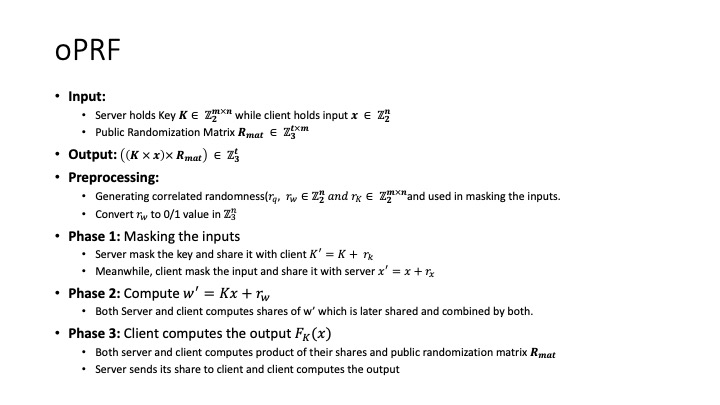
\includegraphics[width=0.8\textwidth]{images/oprf.jpg}
	\vspace{-2mm}
	\caption{oPRF protocol}
	\label{oprf.fig}
	\vspace{-5mm}
\end{figure*}


\begin{algorithm}
	\caption{2-Party oPRF}
	\begin{algorithmic}
		
		\STATE Preprocessing
		
		\STATE Stage\ 1: calculate $a \times b \plus c$
		
		\STATE Stage\ 2: Oblivious Transfer
		
		\STATE stage 3: $Z_3$ randomization  
		
	\end{algorithmic}
\end{algorithm}

\fi






